\documentclass{beamer}
% \usetheme{Boadilla}
\usepackage{float}
\usepackage{cases}
\usepackage{tikz}

\title{A Real-Time, Flexible Logging Infrastructure for MonPoly}
\subtitle{Bachelor's Thesis}
\author{Jonas Degelo}
\institute{ETH Zürich}
\date{February 24, 2023}

% \makeatletter
\setbeamertemplate{frametitle}{
    \ifbeamercolorempty[bg]{frametitle}{}{\nointerlineskip}%
    \@tempdima=\textwidth%
    \advance\@tempdima by\beamer@leftmargin%
    \advance\@tempdima by\beamer@rightmargin%
    \begin{beamercolorbox}[sep=0.3cm,center,wd=\the\@tempdima]{frametitle}
        \usebeamerfont{frametitle}%
        \vbox{}\vskip-1ex%
        \if@tempswa\else\csname beamer@ftecenter\endcsname\fi%
        \strut\insertframetitle\strut\par%
        {%
            \ifx\insertframesubtitle\@empty%
            \else%
            {\usebeamerfont{framesubtitle}\usebeamercolor[fg]{framesubtitle}\insertframesubtitle\strut\par}%
            \fi
        }%
        \vskip-1ex%
        \if@tempswa\else\vskip-.3cm\fi% set inside beamercolorbox... evil here...
    \end{beamercolorbox}%
}
\makeatother
\newcommand*{\Until}[1]{\,\mathcal{U}_{#1}\,}
\newcommand*{\Since}[1]{\,\mathcal{S}_{#1}\,}
\newcommand*{\Next}[1]{\tikz\draw[] (0,0) circle (.8ex);_{#1}}
% \newcommand{\Next}{\Circle}
\newcommand*{\Previous}[1]{\tikz\draw[fill] (0,0) circle (.8ex);_{#1}}
% \newcommand{\Previous}{\Circle[f]}
\newcommand*{\Eventually}[1]{\lozenge_{#1}}
\newcommand*{\Once}[1]{\blacklozenge_{#1}}
\newcommand*{\Always}[1]{\square_{#1}}
\newcommand*{\Historically}[1]{\blacksquare_{#1}}
\newcommand*{\Fregex}[1]{\vartriangleright_{#1}}
\newcommand*{\Pregex}[1]{\blacktriangleleft_{#1}}

\newcommand*{\RI}{\operatorname{RI}}
\newcommand*{\RIr}{\operatorname{RI}_{\text{reg}}}
\newcommand*{\ERI}{\operatorname{ERI}}
\newcommand*{\ERIr}{\operatorname{ERI}_{\text{reg}}}


% \newcommand*{\modelsreg}{\stackrel{\mathclap{\normalfont\mbox{reg}}}{\models}}
\newcommand*{\modelsreg}{\models_{\text{r}}}
% \newcommand*{\modelsreg}{\models_{\text{reg}}}

\newcommand{\filter}{\operatorname{filter}}
\newcommand{\filtertrace}{\operatorname{fil-trace}}
\newcommand{\mask}{\operatorname{mask}}

\newcommand*{\Cupmerge}{\,\ddot{\Cup}\,}
\newcommand*{\subseteqmap}{\,\ddot{\subseteq}\,}
\newcommand*{\subsetmap}{\,\ddot{\subset}\,}
\newcommand*{\Cupext}{\,\dot{\Cup}\,}
\newcommand*{\oplusext}{\,\dot{\oplus}\,}

\newcommand{\keys}{\operatorname{k}}

\newcommand{\inveri}{\operatorname{inverseERI}}
\newcommand{\zeroeri}{\operatorname{zeroERI}}

\newcommand*{\nomoreprecise}{\sqsubseteq}
\newcommand*{\matches}{\rightsquigarrow}



\begin{document}

\begin{frame}
\titlepage
\end{frame}

\section{MonPoly}
\subsection{}

\begin{frame}
    \frametitle{MonPoly}
    \begin{itemize}
        \item Runtime Monitor
        \item Metric First Order Temporal Logic (MFOTL)
    \end{itemize}
    
\end{frame}


\section{The Wrapper}

\begin{frame}
    \frametitle{The Wrapper}
    \centering
    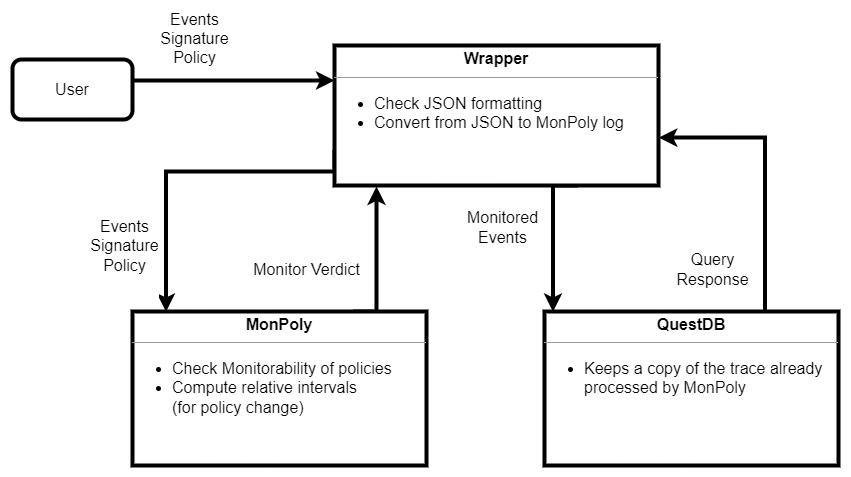
\includegraphics[width=0.9\linewidth]{diagrams/wrapper.png}
\end{frame}

\begin{frame}[fragile]
    \frametitle{Signature to Database Schema 1}

\begin{figure}[H]
    \label{fig:example-signature}
\begin{verbatim}
loc_accessed(user_id: int, purpose: string)
perm_granted(user_id: int)
perm_revoked(user_id: int)
\end{verbatim}
    \caption{Sample MonPoly Signature}
\end{figure}
    
\end{frame}

\begin{frame}[fragile]
    \frametitle{Signature to Database Schema 2}
\begin{figure}[H]
    \label{fig:example-policy-schema}
\begin{verbatim}
CREATE TABLE perm_revoked(x1 INT,
                          time_stamp TIMESTAMP,
                          time_point INT) 
                          timestamp(time_stamp);
CREATE TABLE perm_granted(x1 INT,
                          time_stamp TIMESTAMP,
                          time_point INT) 
                          timestamp(time_stamp);
CREATE TABLE loc_accessed(x1 INT, x2 STRING,
                          time_stamp TIMESTAMP,
                          time_point INT) 
                          timestamp(time_stamp);
CREATE TABLE ts( time_stamp TIMESTAMP,
                 time_point INT) 
                 timestamp(time_stamp);
\end{verbatim}
    \caption{SQL Schema for Sample Policy}
\end{figure}
\end{frame}



\begin{frame}
    \frametitle{Performance Overhead}
    \centering
    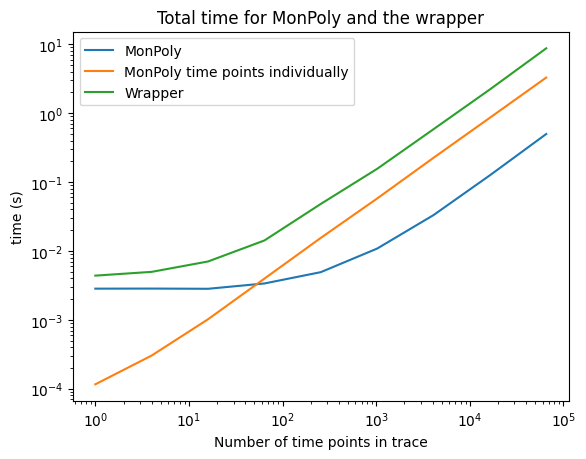
\includegraphics[width=0.9\linewidth]{diagrams/wrapper-monpoly-total.png}
\end{frame}

\section{Algorithm and Policy Change}

\begin{frame}
    \frametitle{Policy Change}
    
\end{frame}

\begin{frame}
    \frametitle{Relative Intervals}
    \begin{definition} 
        \label{def:rel-int}
        The relative interval of the formula $\phi$, $\RI(\phi) \subseteq \mathbb{Z}$ is defined recursively over the formula structure: 
        $\RI(\phi) =$
        \begin{equation*}
            \begin{cases}
                \{0\}     & \text{atomic formula,} \\ 
                \RI(\psi) & \text{$\neg \psi$, 
                                    $\exists x.\psi$,} \\ &\text{or $\forall x.\psi$,} \\
                \RI(\psi) \Cup \RI(\chi) & \text{$\psi \lor \chi, or
                                                \psi \land \chi$,} \\
                (-b,0] \Cup ((-b,-a] \oplus \RI(\psi)) & \text{$\Previous{[a,b)}\psi$,} \\
                [0,b) \Cup ([a,b) \oplus \RI(\psi)) & \text{$\Next{[a,b)}$,}\\
                (-b,0] \Cup ((-b,0] \oplus \RI(\psi)) \Cup ((-b,-a] \oplus \RI(\chi)) & \text{$\psi \Since{}_{[a,b)} \chi$,} \\
                [0,b) \Cup ([0,b) \oplus \RI(\psi)) \Cup ([a,b) \oplus \RI(\chi)) & \text{$\psi \Until{[a,b)} \chi$,} \\
                [0,b) \Cup ([0,b) \oplus \RIr(\rho)) & \text{$\Fregex{[a,b)} \rho$, and}\\
                (-b,0] \Cup ((-b,0] \oplus \RIr(\rho)) & \text{$\Pregex{[a,b)} \rho$.}\\
            \end{cases}
        \end{equation*}
    \end{definition}
\end{frame}

\begin{frame}
    \frametitle{Extended Relative Intervals}

    \begin{definition}
        \label{def:e-rel-int-ops}
        Let $M$ and $N$ be two masked predicate maps and $T$ a positive interval, then 
        \begin{align*}
            M \Cupmerge N = 
                & \{ p(l) \rightarrow (I \Cup J) \mid 
                    p(l) \rightarrow I \in m \text{ and } 
                    p(l) \rightarrow J \in n \} \\
                & \cup \{p(l) \rightarrow I \mid  
                    (p(l) \rightarrow I \in m \text{ and }
                    p(l) \in \keys(M) \setminus \keys(N)) \} \\
                & \cup \{p(l) \rightarrow I \mid  
                    (p(l) \rightarrow I \in n \text{ and }
                    p(l) \in \keys(N) \setminus \keys(M))
                    \} \\
            T \Cupext M = 
                & \{ p(l) \rightarrow (T \Cup I) \mid 
                    p(l) \rightarrow I \in M \} \\
            T \oplusext M = 
                & \{ p(l) \rightarrow (T \oplus I) \mid 
                    p(l) \rightarrow I \in M \} \\
        \end{align*}
    \end{definition}
    
\end{frame}

\begin{frame}
    \frametitle{Extended Relative Intervals}
    \begin{definition}
        \label{def:e-rel-int}
        The extended relative interval of the formula $\varphi$, $\ERI(\varphi)$ is defined recursively over the formula structure:
        $\ERI(\varphi) =$
        \begin{equation*}
            \begin{cases}
                \{\} 
                    & \text{if } \varphi \text{ is an atomic formula} \\
                    & \text{and not a predicate,} \\ 
                \{p(m) \rightarrow [0,0]\} 
                    & \text{if } \varphi \text{ is a predicate with name } \\
                    & p \text{ and mask } m, \\
                \ERI(\psi) 
                    & \text{if } \varphi \text{ is of the form } \neg \psi, \exists x.\psi, \\
                    & \text{or } \forall x.\psi, \\
                \dots
                % \ERI(\psi) \Cupmerge \ERI(\chi) 
                %     & \text{if } \varphi \text{ is of the form } \psi \lor \chi, \\
                %     & \text{or } \psi \land \chi, \\
                % (-b,0] \Cupext ((-b,-a] \oplusext \ERI(\psi)) 
                %     & \text{if } \varphi \text{ is of the form } \Previous{[a,b)} \psi, \\
                % [0,b) \Cupext ([a,b) \oplusext \ERI(\psi)) 
                %     & \text{if } \varphi \text{ is of the form } \Next{[a,b)} \psi,\\
                % (-b,0] \Cupext ((-b,0] \oplusext \ERI(\psi)) \Cupmerge ((-b,-a] \oplusext \ERI(\chi)) 
                %     & \text{if } \varphi \text{ is of the form } \psi \Since{[a,b)} \chi, \\
                % [0,b) \Cupext ([0,b) \oplusext \ERI(\psi)) \Cupmerge ([a,b) \oplusext \ERI(\chi)) 
                %     & \text{if } \varphi \text{ is of the form } \psi \Until{[a,b)} \chi, \\
                % [0,b) \Cupext ([0,b) \oplusext \ERIr(\psi)) 
                %     & \text{if } \varphi \text{ is of the form } \Fregex{[a,b)} \psi, \text{ and}\\
                % (-b,0] \Cupext ((-b,0] \oplusext \ERIr(\psi)) 
                %     & \text{if } \varphi \text{ is of the form } \Pregex{[a,b)} \psi.
            \end{cases}
        \end{equation*}
    \end{definition}
    
\end{frame}

\section{Outlook}

\begin{frame}
    \frametitle{Partial Policy Change in MonPoly}

    % \begin{verbatim}
    %     NAME[<formula>, <name>]
    % \end{verbatim}
    
\end{frame}

\end{document}